\subsection{System Overview} % (fold)
\label{sub:overviewscalenet}

\idx{ScaleNet} addresses both service and network convergence.
At the lower level, the system supports a multitude of heterogeneous physical and logical network elements of fixed and mobile networks into one single all-IP infrastructure.
Figure~\vref{fig:scalenet-structure} lists some of the protocols that could be used~\cite{SIV08B}.

\begin{figure}[htbp]
  \centering
    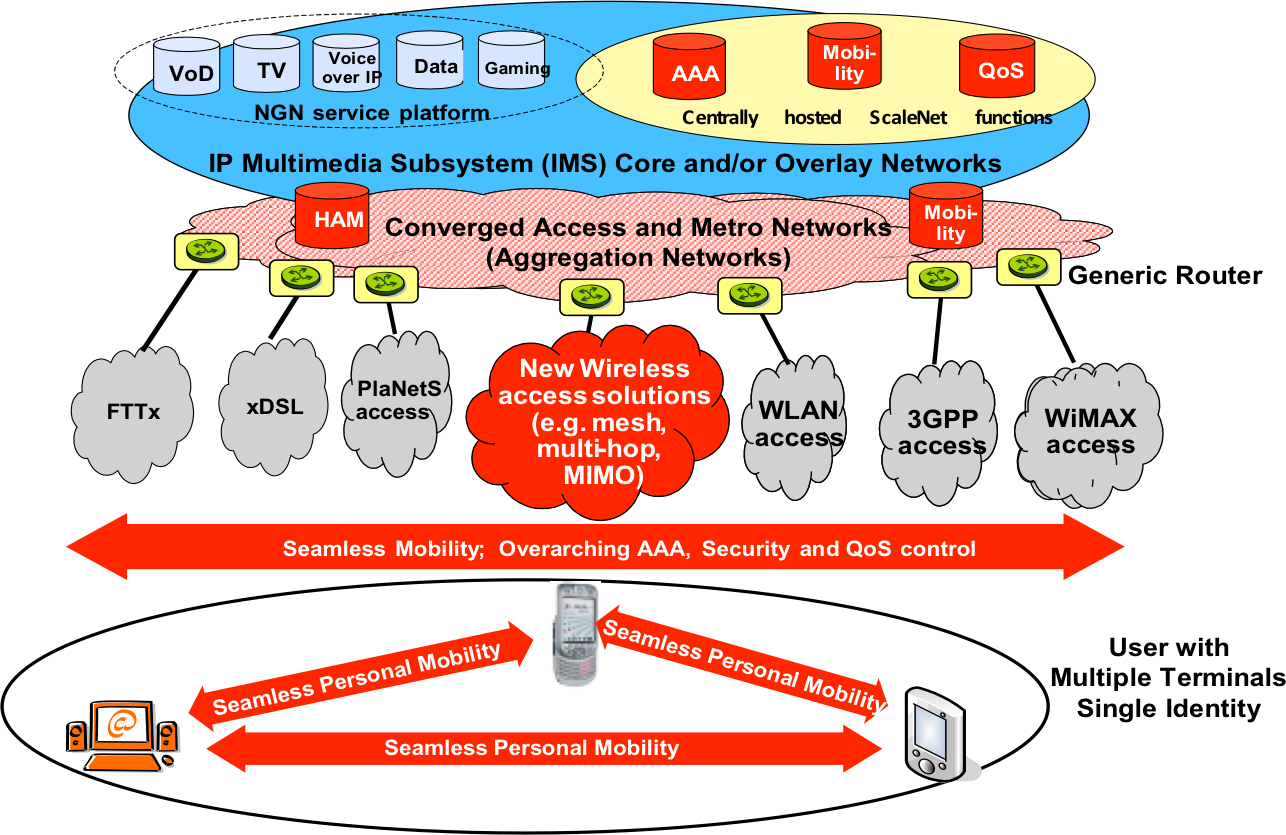
\includegraphics[width=\textwidth]{scalenet-structure}
  \caption{Structure of the system}
  \label{fig:scalenet-structure}
\end{figure}

At an upper level, multimedia services relay on the \ida{IMS} framework for the delivery.
Theoretically \idx{ScaleNet} could support other protocols like Overlay Networks or \ida{P2P}, but \ida{IMS} is the one used by the current implementation.

It is important to notice that the network itself is user-centric, and transparently handles identities by using \ida{SIP}.
This eases supporting users with multiple devices; therefore applications do not have to worry about that part.

It is also important to define what a session means in this system.
A session refers to the current use of a service, so for every service that the user is enjoying a session is created.
For example, if it is viewing a movie but also talking on the \ida{IP} phone, there are two sessions at the same time.

The creation of a session implies that a new service is created, but it goes the other way around too.
If a session is deleted, that service must stop.
If the user ends the service, the session must be deleted.
That means sessions have to be synchronized with the actual services.

A session is also linked to the device that the user is using.
The system allows the copy and transfer of sessions to other devices that he owns, wherever it makes sense.
Since the current implementation has also basic social capabilities, that session can also be transferred or copied to a user's contact.
In the context of this application a user's contact is called ``buddy''.
Figure~\vref{fig:scalenet-structure} lists some of the services that can be offered:

\begin{itemize}
  \item Voice \et{} Video Calls
  \item Mobile TV \et{} \ida{VOD}
  \item \index{MMOG}\acp{MMOG}
  \item Internet Access
\end{itemize}

The work described in this document is primarily focused on the second application, i.e., video streaming.
The idea is that the user can buy a video and play it anywhere using any supported device.

% subsection overviewscalenet (end)